\graphicspath{{4perm/asy/}}
\setcounter{section}{3}

\section{Permutations and Orbits}\label{chap:perm}

In this chapter we return to the origins of group theory by considering the ways in which a set may be reordered.

\subsection{The Symmetric Group, Cycle Notation \& Cayley's Theorem}\label{sec:perm1}

\begin{defn}{}{}
	Let $A$ be a set. A \emph{permutation} of $A$ is a bijective/invertible function $\sigma:A\to A$.\smallbreak
	The \emph{symmetric group} $S_A$ is the set of all permutations of $A$ under functional composition.\smallbreak
	The \emph{symmetric group on $n$-letters\footnotemark} $S_n$ is the group $S_A$ when $A=\{1,2,\ldots,n\}$.
\end{defn}

\footnotetext{%
	This choice of $A$ makes $S_n$ explicit. In practice, any set with $n$ elements will do and any group isomorphic to this is usually also called $S_n$ (see Exercise \ref{exs:symmwd} and the remark regarding ``up to isomorphism" on Page \pageref{sec:uptoiso}).
}


\begin{examples}{}{snbasic}
	\exstart If $A=\{1\}$, there is only one (bijective) function $A\to A$, namely the \emph{identity function} $e:1\mapsto 1$. Thus $S_1$ has only one element and is isomorphic to $\Z_1$.
	\begin{enumerate}\setcounter{enumi}{1}\itemsep0pt
	  \item If $A=\{1,2\}$, then there are \emph{two} bijections $e,\mu:A\to A$:\par
	  \begin{minipage}[t]{0.7\linewidth}\vspace{-10pt}
	    \begin{itemize}\itemsep0pt
	    	\item $e(1)=1$ and $e(2)=2$ defines the identity function.
	    	\item $\sigma(1)=2$ and $\sigma(2)=1$ swaps the elements of $A$.
	  	\end{itemize}
	  \end{minipage}\hfill\begin{minipage}[t]{0.29\linewidth}\vspace{-18pt}
	  \flushright%
	  $\begin{array}{c||c|c}
	  	\circ&e&\sigma\\\hline\hline
	 	 	e&e&\sigma\\\hline
	  	\sigma&\sigma&e
	  \end{array}$
	  \end{minipage}\par
	
	  The Cayley table is immediate: plainly $S_2$ is isomorphic to $\Z_2$.
	  
	  \item\label{ex:snbasic3} $S_3=S_{\{1,2,3\}}$ has \emph{six elements} and is \emph{non-abelian}. We have met this group before: note how every rotation/reflection of the triangle in Example \ref{ex:d3} corresponds to a permutation of the three vertices 1, 2, 3. Otherwise said, $S_3$ is isomorphic to the dihedral group $D_3$. 
	\end{enumerate}
\end{examples}

\begin{lemm}{}{sabasic}
	\exstart $S_A$ is a group under composition of functions.\vspace{-4pt}
	\begin{enumerate}\setcounter{enumi}{1}\itemsep0pt
	  \item If $A$ has at least three elements, then $S_A$ is non-abelian.
	  \item The order of $S_n$ is $n!$ \hfill (\textcolor{red}{Warning!} The order of $S_n$ is \textcolor{red}{not} the subscript $n$)
	  \item $S_m\le S_n$ whenever $m\le n$ \hfill(Strictly, $S_n$ contains a subgroup \emph{isomorphic} to $S_m$)
	\end{enumerate}
\end{lemm}

\begin{proof}
	\exstart The axioms follow from familiar function properties. Write out the details if you're unsure.\vspace{-5pt}
  \begin{quote}
		\emph{Closure}: \ If $\sigma,\tau:A\to A$ are bijective, so is the composition $\sigma\circ\tau$.\par
		\emph{Associativity}: \ Composition of functions is associative (Exercise \ref*{sec:geomgroups}.\ref{exs:funcassoc}).\par
		\emph{Identity}: \ The \emph{identity function} $e_A:a\mapsto a$ for all $a\in A$ is certainly bijective.\par
		\emph{Inverse}: \ If $\sigma$ is a bijection, then its inverse function $\sigma^{-1}$ is also bijective.
	\end{quote}
		The remaining parts are exercises.
\end{proof}

From now on we use juxtaposition: $\sigma\tau:=\sigma\circ\tau$. Exponentiation therefore means self-composition: e.g.\ $\sigma^3=\sigma\sigma\sigma=\sigma\circ\sigma\circ\sigma$. Remember also that $\sigma\tau$ is a \emph{function} $A\to A$, and that evaluation means that we act with $\tau$ first:
\[
	\forall a\in A, \ \sigma\tau(a)=\sigma\bigl(\tau(a)\bigr)
\]


\goodbreak


% \begin{minipage}[t]{0.7\linewidth}\vspace{0pt}
% 	\emph{\textcolor{red}{Standard notation}} simply copies the table with different formatting.
% \end{minipage}\begin{minipage}[t]{0.3\linewidth}\vspace{0pt}
% 	\flushright$\textcolor{red}{\sigma=\begin{pmatrix}
%          1&2&3&4\\
%          3&1&4&2
% 	\end{pmatrix}}$
% \end{minipage}\medbreak
%          
% \begin{minipage}[t]{0.46\linewidth}\vspace{0pt}
% 	\emph{\textcolor{Green}{Matrix notation}} views $\sigma$ as a \emph{permutation matrix}; a square matrix with a single 1 in each row/column and which acts by multiplication on the input viewed as a column vector. Composition of permutations is simply matrix multiplication.
% \end{minipage}\hfill\begin{minipage}[t]{0.52\linewidth}\vspace{0pt}
% $\begin{pmatrix}
%          0&0&1&0\\
%          1&0&0&0\\
%          0&0&0&1\\
%          0&1&0&0
%          \end{pmatrix}\fourvec 1234=\fourvec 3142$ \hfill \textcolor{Green}{$\sigma=\begin{pmatrix}
%          0&0&1&0\\
%          1&0&0&0\\
%          0&0&0&1\\
%          0&1&0&0
%          \end{pmatrix}$}
% \end{minipage}\bigbreak


\boldsubsubsection{Cycle Notation}

Efficient computation in $S_n$ is facilitated by some new notation.

\begin{defn}{}{cycle}
	Suppose $\{a_1,\ldots,a_k\}\subseteq\{1,\ldots,n\}$. The \emph{$k$-cycle} $\sigma=(a_1\ a_2\cdots a_k)\in S_n$ is the function\par
	\begin{minipage}[t]{0.5\linewidth}\vspace{-12pt}
	\[
		\sigma:
		\begin{cases}
			a_j\mapsto a_{j+1}&\text{if $j<k$}\\
			a_k\mapsto a_1\\
			x\mapsto x&\text{if }x\not\in\{a_1,\ldots,a_k\}
		\end{cases}
	\]
	\end{minipage}
	\hfill
	\begin{minipage}[t]{0.49\linewidth}\vspace{2pt}
		\flushright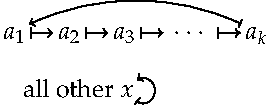
\includegraphics[scale=0.9]{perm-cycle4}
	\end{minipage}\bigbreak
	Cycles $(a_1\cdots a_k)$ and $(b_1\cdots b_l)$ are \emph{disjoint} if $\{a_1,\ldots,a_k\}\cap\{b_1,\ldots,b_l\}=\emptyset$.\smallbreak
	\emph{1-cycles} and the \emph{0-cycle} $()$ can be helpful in calculations, though both are simply the identity $e$.
\end{defn}

\begin{example}{}{cyclebasic}
	A 4-cycle $\textcolor{blue}{\sigma=(1\,3\,4\,2)}$ and a 2-cycle $\textcolor{red}{\tau=(1\,4)}$ in $S_4$ are defined in the table:
	\[
		\begin{array}[t]{c||cccc}
			x&1&2&3&4\\\hline\hline
			\textcolor{blue}{\sigma}(x)&3&1&4&2\\\hline
			\textcolor{red}{\tau}(x)&4&2&3&1
		\end{array}
		\qquad\qquad
		\SelectTips{cm}{}
		\xymatrix @C15pt @R5pt{%
			&&&\\
		 	\makebox[0pt][r]{$\textcolor{blue}{\sigma}:\ $}1 \ar@{|->}@[blue][r] & 3 \ar@{|->}@[blue][r] & 4 \ar@{|->}@[blue][r] & 2 \ar@/_1.0pc/@<-2pt>@{|->}@[blue][lll]
		}
		\qquad\qquad
		\SelectTips{cm}{}
		\xymatrix @C15pt @R5pt{%
			&&&\\
		 	\makebox[0pt][r]{$\textcolor{red}{\tau}:$\ }1 \ar@/_0.8pc/@{|->}@[red][r]& 4 \ar@/_0.8pc/@{|->}@[red][l] & 2 \ar@{|->}@(dr,ur)@[red] & 3 \ar@{|->}@(dr,ur)@[red]
		}
	\]
	To compose cycles, remember that both are \emph{functions} and you won't go wrong!
	\[
		\begin{array}[t]{c|cccc}
			x&1&2&3&4\\\hline
			\tau(x)&4&2&3&1\\\hline
			\sigma\tau(x)&2&1&4&3
		\end{array}
		\qquad\qquad
		\SelectTips{cm}{}
		\xymatrix @C12pt @R5pt{%
			&&&\\
	 		\makebox[0pt][r]{$\sigma\tau:$\ }1 \ar@/_0.8pc/@{|->}[r] & 2 \ar@/_0.8pc/@{|->}[l] & 3 \ar@/_0.8pc/@{|->}[r] & 4 \ar@/_0.8pc/@{|->}[l]
		}
	\]
	The result is a product of \emph{disjoint 2-cycles} $\sigma\tau=(1\,2)(3\,4)$.
\end{example}



\boldinline{Algorithmic Cycle Composition}\phantomsection\label{pg:cyclenot}

Computation using tables is impractically slow. Here is an algorithmic approach that, with practice, should prove more efficient. We illustrate by verifying the previous calculation: at each stage we write only a \textcolor{red}{single number or bracket}, building up the right column below.

\begin{itemize}\itemsep0pt
  \item Open a \textcolor{red}{bracket} and write \textcolor{red}{1}.\hfill $\sigma\tau=\textcolor{red}{(1}\phantom{\,2)(3\,4)}$
  \item Since $1\overset{\tau}{\mapsto}4\overset{\sigma}{\mapsto}2$, we next write \textcolor{red}{2}.\hfill $=(1\,\textcolor{red}{2}\phantom{)(3\,4)}$
  \item $2\overset{\tau}{\mapsto}2\overset{\sigma}{\mapsto}1$ restarts the cycle; \textcolor{red}{close it} and start another with an \textcolor{red}{unused value}.\hfill $=(1\,2\textcolor{red}{)(3}\phantom{\,4)}$
  \item $3\overset{\tau}{\mapsto}3\overset{\sigma}{\mapsto}4$, so next write \textcolor{red}{4}.\hfill $=(1\,2)(3\,\textcolor{red}{4}\phantom{)}$
  \item $4\overset{\tau}{\mapsto}1\overset{\sigma}{\mapsto}3$ restarts the current cycle, so \textcolor{red}{close it}.\hfill $=(1\,2)(3\,4\textcolor{red}{)}$
  \item All values 1, 2, 3, 4 have appeared so the algorithm terminates.
\end{itemize}
It should be clear how to extend the algorithm when composing more cycles. Any 1-cycles obtain should be deleted. Shortly we'll prove that the algorithm always terminates in a product of disjoint cycles (Theorem \ref{thm:cycleterminates}). For now, practice it by verifying the following:

\begin{examples}{}{}
	\exstart $(1\,4)(1\,3\,4\,2)=(1\,3)(2\,4)$\hfill \makebox[230pt][l]{2.\lstsp$(1\,3\,5\,4)(2\,3\,4)=(1\,3)(2\,5\,4)$}
	\begin{enumerate}\setcounter{enumi}{2}
	  \item $(1\,2\,3\,4)(1\,2\,3)(1\,2)=(1\,4)(2\,3)$\hfill \makebox[230pt][l]{4.\lstsp$(1\,2\,3\,4\,5\,6)^3=(1\,4)(2\,5)(3\,6)$}
	\end{enumerate}
\end{examples}


\goodbreak


\boldsubsubsection{Geometric Symmetry Groups (Section \ref{sec:geomgroups} revisited)}

We've already seen (Example \ref*{ex:snbasic}.\ref{ex:snbasic3}) how the symmetry group $D_3$ of an equilateral triangle is isomorphic to the symmetric group $S_3$. The same trick applies more generally: label the vertices (or edges/faces) of a figure with numbers $1,2,3,\ldots$ and represent each rotation/reflection by how it permutes these values. Cycle notation makes calculating compositions easy!

\begin{examples}{}{disym}
	\exstart Label the edges of a rectangle to view the Klein four-group $V$ as a subgroup of $S_4$: the 2-cycles $(1\,3)$ and $(2\,4)$ are reflections, and their composition is rotation by \ang{180}.
	\[
		\begin{minipage}{0.36\textwidth}\vspace{-3pt}
			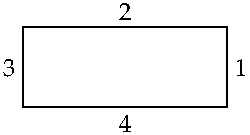
\includegraphics[scale=0.9]{perm-rect}
		\end{minipage}\qquad
		\displaystyle V\cong\bigl\{e,(1\,3),(2\,4),(1\,3)(2\,4)\bigr\}
	\]
	Alternative descriptions of $V$ can be obtained by using different labellings (Exercise \ref{exs:kleins4}).
	
	\begin{enumerate}\setcounter{enumi}{1}
		\begin{minipage}[t]{0.77\linewidth}\vspace{-8pt}
			\item Label the vertices of a regular hexagon 1 through 6.
		  \begin{itemize}
		  	\item The 2,2-cycle $(1\,5)(2\,4)$ represents reflection across the line through 3 and 6.
		  	\item The 6-cycle $(1\,2\,3\,4\,5\,6)$ represents \ang{60} counter-clockwise rotation.
			\end{itemize}
		\end{minipage}
		\hfill
		\begin{minipage}[t]{0.22\linewidth}\vspace{-10pt}
			\flushright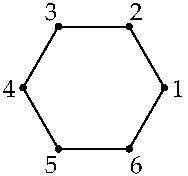
\includegraphics[scale=0.95]{perm-hexagon}
		\end{minipage}\smallbreak
		Both functions describe elements of the dihedral group $D_6$. By extension, $D_6$ may be identified as (is isomorphic to) a subgroup of $S_6$.
	
		\begin{minipage}[t]{0.77\linewidth}\vspace{0pt}
			\item By labelling the vertices of a square, we may identify $D_4$ with a subgroup of $S_4$. All elements and the complete subgroup diagram are given below. By convention we denote reflections across diagonals ($\delta_j$) and the midpoints of sides ($\mu_j$) differently.\smallbreak
			Note the ease of computations: e.g.,
			\[
				(2\,4)(1\,2)(3\,4)=(1\,4\,3\,2)\implies \delta_1\mu_1=\rho_3
			\]
		\end{minipage}
		\hfill
		\begin{minipage}[t]{0.22\linewidth}\vspace{0pt}
			\flushright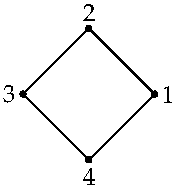
\includegraphics[scale=0.95]{perm-d4}
		\end{minipage}\medbreak
	
	%\begin{minipage}[t]{.5\linewidth}\vspace{0pt}
	% \[\def\arraystretch{1.1}\begin{array}{c||c|c|c|c|c|c|c|c}
	% \circ & \rho_0 & \rho_1 & \rho_2 &\rho_3 & \mu_1 & \mu_2 & \delta_1 & \delta_2\\
	%  \hline\hline
	% \rho_0 & \rho_0 & \rho_1 & \rho_2 & \rho_3 & \mu_1 & \mu_2 & \delta_1 & \delta_2\\
	% \hline
	% \rho_1 & \rho_1 & \rho_2 & \rho_3 & \rho_0 & \delta_2 & \delta_1 & \mu_1 & \mu_2\\
	% \hline
	% \rho_2 & \rho_2 & \rho_3 & \rho_0 & \rho_1 & \mu_2 & \mu_1 & \delta_2 & \delta_1\\
	% \hline
	% \rho_3 & \rho_3 & \rho_0 & \rho_1 & \rho_2 & \delta_1 & \delta_2 & \mu_2 & \mu_1\\
	% \hline
	% \mu_1 & \mu_1 & \delta_1 & \mu_2 & \delta_2 & \rho_0 & \rho_2 & \rho_1 & \rho_3\\
	% \hline
	% \mu_2 & \mu_2 & \delta_2 & \mu_1 & \delta_1 & \rho_2 & \rho_0 & \rho_3 & \rho_1\\
	% \hline
	% \delta_1 & \delta_1 & \mu_2 & \delta_2 & \mu_1 & \rho_3 & \rho_1 & \rho_0 & \rho_2\\
	% \hline
	% \delta_2 & \delta_2 & \mu_1 & \delta_1 & \mu_2 & \rho_1 & \rho_3 & \rho_2 & \rho_0
	% \end{array}\]
	%\end{minipage}
	
			
	\begin{minipage}[t]{\linewidth}\vspace{0pt}
		\begin{minipage}[t]{.3\linewidth}\vspace{0pt}
			\def\arraystretch{1.1}
			\begin{tabular}{|r|c|c|}\hline
		    \multicolumn{2}{|c|}{Element} & Cycle notation\\\hline
		    & $\rho_0$ & $e=()$\\\cline{2-3}
		    \multirow{2}{*}{\rotatebox{90}{\smash[b]{\makebox[0cm]{\ Rotations}}}} & $\rho_1$ & $(1234)$\\\cline{2-3}
		    & $\rho_2$ & $(13)(24)$\\\cline{2-3}
		    & $\rho_3$ & $(1432)$\\\hline
		    & $\mu_1$ & $(12)(34)$\\\cline{2-3}
		    \multirow{2}{*}{\rotatebox{90}{\smash[b]{\makebox[0cm]{\ \,Reflections}}}} & $\mu_2$ & $(14)(23)$\\\cline{2-3}
		    & $\delta_1$ & $(24)$\\\cline{2-3}
		    & $\delta_2$ & $(13)$\\\hline
		  \end{tabular}
		\end{minipage}
		\hfill
		\begin{minipage}[t]{.3\linewidth}\vspace{0pt}
		  \def\arraystretch{1.1}
		  $\begin{array}{|c|c|c|}\hline
		    \text{Subgroup} & \text{Isomorph}\\\hline
		     \{\rho_0\} & \Z_1\\\hline
		     \textcolor{red}{\{\rho_0,\mu_i\}} & \textcolor{red}{\Z_2}\\\hline
		     \textcolor{blue}{\{\rho_0,\delta_i\}} & \textcolor{blue}{\Z_2}\\\hline
		     \{\rho_0,\rho_2\} & \Z_2\\\hline
		     \{\rho_0,\rho_1,\rho_2,\rho_3\} & \Z_4\\\hline
		     \textcolor{red}{\{\rho_0,\mu_1,\mu_2,\rho_2\}} & \textcolor{red}{V}\\\hline
		     \textcolor{blue}{\{\rho_0,\delta_1,\delta_2,\rho_2\}} & \textcolor{blue}{V}\\\hline
		  \end{array}$
		\end{minipage}
		\hfill
		\begin{minipage}[t]{.31\linewidth}\vspace{0pt}
			$\xymatrix @R18pt @C10pt{%
				&& D_4 \ar@{-}[dl] \ar@{-}[d] \ar@{-}[dr] &&\\
				& \textcolor{red}{V} \ar@{-}[dr] \ar@{-}[d] \ar@{-}[dl] & \Z_4 \ar@{-}[d] & \textcolor{blue}{V} \ar@{-}[dr] \ar@{-}[d] \ar@{-}[dl] & \\
				\textcolor{red}{\Z_2} \ar@{-}[drr] & \textcolor{red}{\Z_2} \ar@{-}[dr] & \Z_2 \ar@{-}[d] & \textcolor{blue}{\Z_2} \ar@{-}[dl] & \textcolor{blue}{\Z_2} \ar@{-}[dll] \\
				&& \Z_1 &&
			}$
		\end{minipage}
	\end{minipage}\par
	
	You should be able to recognize these subgroups geometrically; e.g.\ the blue copy of $\textcolor{blue}{V}$ is precisely that in the first example! Try to convince yourself why there are no other subgroups.
	\end{enumerate}
\end{examples}
The same thing can be done for 3D figures like the tetrahedron (Example \ref*{ex:tetra}.\ref{ex:tetra2}).

\goodbreak

% TIDY AND SIMPLIFY FROM HERE
% 
% \boldinline{Elements of $D_n$} The regular $n$-gon has $2n$ distinct symmetries and so $\nm{D_n}=2n$. These consist of:
% \begin{description}
% \item[$n$ rotations] For each $j=0,\ldots,n-1$, let $\rho_j$ be rotation counter-clockwise by $\frac{2\pi j}{n}$ radians. 
% \item[$n$ reflections] Let $\mu_j$ be reflection across the line making angle $\frac{\pi j}{n}$ with the positive $x$-axis (make sure you put one of the corners of the $n$-gon on the $x$-axis!).\footnote{For \emph{even}-sided polygons these are often labelled differently, and split into two subsets of $\frac n2$ reflections each. The reflections $\mu_i$ are those which move \emph{all} the corners of the $n$-gon, while $\delta_i$ refers to a reflection across a \emph{diagonal.} We will see this in our treatment of $D_4$ below. In the abstract, is is simpler not to distinguish between these reflections.}
% \end{description}
% 
% \boldinline{Remarks}
% Some authors write $D_{2n}$ instead of $D_n$ precisely because $\nm{D_n}=2n$: in this course, $D_n$ will \emph{always} mean the symmetries of the $n$-gon.\\
% Every dihedral group $D_n$ is a subgroup of the orthogonal group $\rO_2(\R)$. The correspondence is:
% \[\rho_j=\begin{pmatrix}
%          \cos\left(\frac{2\pi j}{n}\right)&-\sin\left(\frac{2\pi j}{n}\right)\\ \sin\left(\frac{2\pi j}{n}\right)&\cos\left(\frac{2\pi j}{n}\right)
%          \end{pmatrix}\qquad\qquad \mu_j=\begin{pmatrix}
%          \cos\left(\frac{2\pi j}{n}\right)&\sin\left(\frac{2\pi j}{n}\right)\\ \sin\left(\frac{2\pi j}{n}\right)&-\cos\left(\frac{2\pi j}{n}\right)
%          \end{pmatrix}\]
% It is a good exercise to convince yourself that these matrices really do correspond to the rotations and reflections claimed. In particular multiply any two of them together and see what you get\ldots


% \subsubsection*{Subgroup relations between dihedral groups}
% 
% $D_m\le D_n\iff m\mid n$. Recall the discussion of %\hyperlink{sec:geomdih}{geometric proofs:}%
% geometric proofs earlier where we saw that $D_3\le D_6$. For instance, we can join every $(n/m)^{\text{th}}$ vertex of a regular $n$-gon to obtain a regular $m$-gon. Every symmetry of the $m$-gon is then a symmetry of the $n$-gon.
% 
% 
% \subsubsection*{Explicit descriptions of $D_3$ and $D_4$}
% 
% \begin{minipage}{.75\linewidth}
% $D_3$ is the group of symmetries of an equilateral triangle. If we label the corners as in the picture, we can easily define the elements of the group.
% \begin{description}\itemsep0pt
% \item[$\rho_0$] the identity
% \item[$\rho_1$] rotate counter-clockwise by $\frac{2\pi}3$ radians
% \item[$\rho_2$] rotate clockwise by $\frac{2\pi}3$ radians
% \item[$\mu_i$] reflect in the altitude through $i$
% \end{description}
% \end{minipage}\begin{minipage}{.25\textwidth}\vspace{0pt}
% \flushright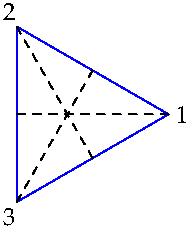
\includegraphics{perm-d3}
% \end{minipage}\par
% Here we write all the elements in permutation notation ad give the Cayley table.\label{pg:d3}
% 
% \begin{minipage}[t]{.46\linewidth}\vspace{0pt}
% \[\def\arraystretch{1.5}\begin{array}{c||c|c|c|c|c|c}
% \circ & \rho_0 & \rho_1 & \rho_2 & \mu_1 & \mu_2 & \mu_3\\
%  \hline\hline
% \rho_0 & \rho_0 & \rho_1 & \rho_2 & \mu_1 & \mu_2 & \mu_3\\
% \hline
% \rho_1 & \rho_1 & \rho_2 & \rho_0 & \mu_3 & \mu_1 & \mu_2\\
% \hline
% \rho_2 & \rho_2 & \rho_0 & \rho_1 & \mu_2 & \mu_3 & \mu_1\\
% \hline
% \mu_1 & \mu_1 & \mu_2 & \mu_3 & \rho_0 & \rho_1 & \rho_2\\
% \hline
% \mu_2 & \mu_2 & \mu_3 & \mu_1 & \rho_2 & \rho_0 & \rho_1\\
% \hline
% \mu_3 & \mu_3 & \mu_1 & \mu_2 & \rho_1 & \rho_2 & \rho_0
% \end{array}\]
% \end{minipage}\begin{minipage}[t]{.5\linewidth}\vspace{0pt}
% \begin{tabular}{|r|c|c|c|}\hline
%     \multicolumn{2}{|c|}{Element} & Standard notation & Cycle notation\\\hline
%     \multirow{5}{*}{\rotatebox{90}{\smash[b]{\makebox[0cm]{Rotations}}}}
%      & $\rho_0$ & $\begin{pmatrix} 1&2&3\\1&2&3 \end{pmatrix}$ & $e=()$\\\cline{2-4}
%    & $\rho_1$ & $\begin{pmatrix} 1&2&3\\2&3&1 \end{pmatrix}$ & $(123)$\\\cline{2-4}
%     & $\rho_2$ & $\begin{pmatrix} 1&2&3\\3&1&2 \end{pmatrix}$ & $(132)$\\\hline
%     \multirow{5}{*}{\rotatebox{90}{\smash[b]{\makebox[0cm]{Reflections}}}} & $\mu_1$ & $\begin{pmatrix} 1&2&3\\1&3&2 \end{pmatrix}$ & $(23)$\\\cline{2-4}
%     & $\mu_2$ & $\begin{pmatrix} 1&2&3\\3&2&1 \end{pmatrix}$ & $(13)$\\\cline{2-4}
%     & $\mu_3$ & $\begin{pmatrix} 1&2&3\\2&1&3 \end{pmatrix}$ & $(12)$\\\hline
%   \end{tabular}
% \end{minipage}\par
% 
% It should be immediately obvious that all the permutations of $\{1,2,3\}$ are elements of $D_3$, and so $D_3\cong S_3$. Now we consider all the subgroups of $D_3$ and its subgroup diagram.\par
% 
% \begin{minipage}{.6\linewidth}
% \qquad$\begin{array}{|c|c|c|}\hline
%     \text{Subgroup} & \text{Isomorph} & \text{Generating sets}\\\hline
%      \{\rho_0\} & C_1 & \{\rho_0\}\\\hline
%      \{\rho_0,\mu_1\} & C_2 & \{\mu_1\}\\\hline
%      \{\rho_0,\mu_2\} & C_2 & \{\mu_2\}\\\hline
%      \{\rho_0,\mu_3\} & C_2 & \{\mu_3\}\\\hline
%      \{\rho_0,\rho_1,\rho_2\} & C_3 & \{\rho_1\},\text{ or }\{\rho_2\}\\\hline
%      D_3 & S_3 & \text{\parbox[c]{3.9cm}{any pair $\{\rho_i,\mu_j\}$ where $i=1,2$ and $j=1,2,3$}}\\\hline
%   \end{array}$
% \end{minipage}\hfill\begin{minipage}{.36\linewidth}
% $\xymatrix @R35pt @C20pt{ & D_3 \ar@{-}[dl] \ar@{-}[d] \ar@{-}[dr] \ar@{-}[drr] &&\\
% C_3 \ar@{-}[dr] & C_2 \ar@{-}[d] & C_2 \ar@{-}[dl] & C_2 \ar@{-}[dll] \\
% & C_1 & &}$
% \end{minipage}\par
% 
% How can we be certain that there are no other subgroups of $D_3$? A careful consideration of generating sets should convince you. For example, suppose that a subgroup contains two reflections: WLOG suppose these are $\mu_1,\mu_2$. We compute the subgroup generated by $\{\mu_1,\mu_2\}$. It must include
% \begin{gather*}
% \mu_1\mu_2=\rho_1,\qquad
% \rho_1^2=\rho_2\qquad
% \mu_1\rho_1=\mu_3
% \end{gather*}
% and thus the entire group.
% 
% \begin{minipage}{.7\linewidth}
% $D_4$ is the group of symmetries of the square. It consists of four rotations and four reflections: the notation $\delta_j$ for reflection across a diagonal is used here, rather than labelling all reflections $\mu_j$.
% \begin{description}\itemsep0pt
% \item[$\rho_0$] the identity
% \item[$\rho_1$] rotate counter-clockwise by $\frac{\pi}2$ radians
% \item[$\rho_2$] rotate counter-clockwise by $\pi$ radians
% \item[$\rho_3$] rotate counter-clockwise by $\frac{3\pi}2$ radians
% \item[$\mu_i$] reflect across midpoints of sides
% \item[$\delta_i$] reflect across diagonals
% \end{description}
% \end{minipage}\begin{minipage}{.3\textwidth}\vspace{0pt}
% \flushright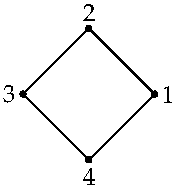
\includegraphics{perm-d4}
% \end{minipage}
% 
% \begin{minipage}[t]{.5\linewidth}\vspace{0pt}
% \[\def\arraystretch{1.5}\begin{array}{c||c|c|c|c|c|c|c|c}
% \circ & \rho_0 & \rho_1 & \rho_2 &\rho_3 & \mu_1 & \mu_2 & \delta_1 & \delta_2\\
%  \hline\hline
% \rho_0 & \rho_0 & \rho_1 & \rho_2 & \rho_3 & \mu_1 & \mu_2 & \delta_1 & \delta_2\\
% \hline
% \rho_1 & \rho_1 & \rho_2 & \rho_3 & \rho_0 & \delta_2 & \delta_1 & \mu_1 & \mu_2\\
% \hline
% \rho_2 & \rho_2 & \rho_3 & \rho_0 & \rho_1 & \mu_2 & \mu_1 & \delta_2 & \delta_1\\
% \hline
% \rho_3 & \rho_3 & \rho_0 & \rho_1 & \rho_2 & \delta_1 & \delta_2 & \mu_2 & \mu_1\\
% \hline
% \mu_1 & \mu_1 & \delta_1 & \mu_2 & \delta_2 & \rho_0 & \rho_2 & \rho_1 & \rho_3\\
% \hline
% \mu_2 & \mu_2 & \delta_2 & \mu_1 & \delta_1 & \rho_2 & \rho_0 & \rho_3 & \rho_1\\
% \hline
% \delta_1 & \delta_1 & \mu_2 & \delta_2 & \mu_1 & \rho_3 & \rho_1 & \rho_0 & \rho_2\\
% \hline
% \delta_2 & \delta_2 & \mu_1 & \delta_1 & \mu_2 & \rho_1 & \rho_3 & \rho_2 & \rho_0
% \end{array}\]
% \end{minipage}\begin{minipage}[t]{.5\linewidth}\vspace{0pt}
% \begin{tabular}{|r|c|c|c|}\hline
%     \multicolumn{2}{|c|}{Element} & Standard notation & Cycle notation\\\hline
%     & $\rho_0$ & $\begin{pmatrix} 1&2&3&4\\1&2&3&4 \end{pmatrix}$ & $e=()$\\\cline{2-4}
%     \multirow{3}{*}{\rotatebox{90}{\smash[b]{\makebox[0cm]{Rotations}}}} & $\rho_1$ & $\begin{pmatrix} 1&2&3&4\\2&3&4&1 \end{pmatrix}$ & $(1234)$\\\cline{2-4}
%     & $\rho_2$ & $\begin{pmatrix} 1&2&3&4\\3&4&1&2 \end{pmatrix}$ & $(13)(24)$\\\cline{2-4}
%     & $\rho_3$ & $\begin{pmatrix} 1&2&3&4\\4&1&2&3 \end{pmatrix}$ & $(1432)$\\\hline
%     & $\mu_1$ & $\begin{pmatrix} 1&2&3&4\\2&1&4&3 \end{pmatrix}$ & $(12)(34)$\\\cline{2-4}
%     \multirow{3}{*}{\rotatebox{90}{\smash[b]{\makebox[0cm]{Reflections}}}} & $\mu_2$ & $\begin{pmatrix} 1&2&3&4\\4&3&2&1 \end{pmatrix}$ & $(14)(23)$\\\cline{2-4}
%     & $\delta_1$ & $\begin{pmatrix} 1&2&3&4\\1&4&3&2 \end{pmatrix}$ & $(24)$\\\cline{2-4}
%     & $\delta_2$ & $\begin{pmatrix} 1&2&3&4\\3&2&1&4 \end{pmatrix}$ & $(13)$\\\hline
%   \end{tabular}
% \end{minipage}\par
% 
% All the subgroups are summarised in the following table. In particular, note that $D_4\ncong S_4$: the latter has many more elements!
% 
% \begin{minipage}{.63\linewidth}
%   $\begin{array}{|c|c|c|}\hline
%     \text{Subgroup} & \text{Isomorph} & \text{Generating sets}\\\hline
%      \{\rho_0\} & C_1 & \{\rho_0\}\\\hline
%      \{\rho_0,\mu_i\} & C_2 & \{\mu_i\}\text{ for each $i$}\\\hline
%      \{\rho_0,\delta_i\} & C_2 & \{\delta_i\}\text{ for each $i$}\\\hline
%      \{\rho_0,\rho_2\} & C_2 & \{\rho_2\}\\\hline
%      \{\rho_0,\rho_1,\rho_2,\rho_3\} & C_4 & \{\rho_1\}\text{ or }\{\rho_3\}\\\hline
%      \{\rho_0,\mu_1,\mu_2,\rho_2\} & V & \{\mu_1,\mu_2\},\ \{\mu_1,\rho_2\}\text{ or }\{\mu_2,\rho_2\}\\\hline
%      \{\rho_0,\delta_1,\delta_2,\rho_2\} & V & \{\delta_1,\delta_2\},\ \{\delta_1,\rho_2\}\text{ or }\{\delta_2,\rho_2\}\\\hline
%      D_4 & D_4 & \text{\parbox[c]{5.4cm}{any pair $\{\rho_i,\mu_j\}$ or $\{\rho_i,\delta_j\}$ where $i=1,3$ and $j=1,2$ or any pair $\{\mu_k,\delta_l\}$ where $k,l=1,2$}}\\\hline
%   \end{array}$
% \end{minipage}\hfill\begin{minipage}{.36\linewidth}
% $\xymatrix @R35pt @C20pt{ && D_4 \ar@{-}[dl] \ar@{-}[d] \ar@{-}[dr] &&\\
% & V \ar@{-}[dr] \ar@{-}[d] \ar@{-}[dl] & C_4 \ar@{-}[d] & V \ar@{-}[dr] \ar@{-}[d] \ar@{-}[dl] & \\
% C_2 \ar@{-}[drr] & C_2 \ar@{-}[dr] & C_2 \ar@{-}[d] & C_2 \ar@{-}[dl] & C_2 \ar@{-}[dll] \\
% && C_1 &&}$
% \end{minipage}\par
% 
% In the subgroup diagram, the middle $C_2$ is $\{\rho_0,\rho_2\}$ while the two copies on each side contain either the reflections $\delta_i$ or $\mu_i$.



\boldsubsubsection{Cayley's Theorem}
   
The word \emph{group}, at least in mathematics, originally referred to a set of permutations. We finish this section with a foundational result that links to the original meaning of the word: every element of a group may be viewed as a permutation---indeed of the group itself!

\begin{thm}{Cayley}{cayley}
	Every group is isomorphic to a group of permutations.
\end{thm}

The proof of Cayley's Theorem is merely the abstraction of a simple example.

\begin{example}{}{}
	To each integer $g$, we may associate the \emph{function} ``add $g$.'' For instance, 1 corresponds to the function ``$+1$,'' etc. The function ``add $g$'' is a bijection of the integers: its inverse function is ``add $-g$.'' Each integer is therefore naturally associated to a \emph{permutation}, an element of the group $S_\Z$.
\end{example}

\begin{proof}
	Let $G$ be a group. For each $g\in G$, define \emph{left-multiplication by $g$} to be the function $L_g:G\to G$ where,
	\[
		\forall x\in G,\ L_g(x)=gx
	\]
	This is bijective (inverse function $(L_g)^{-1}=L_{g^{-1}}$), and therefore a \emph{permutation} of $G$: that is $L_g\in S_G$.\smallbreak
	Now define a function $\phi:G\to S_G$ by $\phi(g)=L_g$. We prove that $\phi$ is an injective homomorphism.
	\begin{description}
		\item[Injectivity] $\phi(g)=\phi(h)\Longrightarrow L_g=L_h\Longrightarrow L_g(e)=L_h(e)\Longrightarrow ge=he\Longrightarrow g=h$
		\item[Homomorphism] We show that $\phi(gh)=\phi(g)\phi(h)$ \emph{as functions} by evaluating on all $x\in G$:
		\[
			\bigl(\phi(gh)\bigr)(x) =L_{gh}(x)=(gh)x=g(hx) =L_g\bigl(L_h(x)\bigr)=\bigl(\phi(g)\phi(h)\bigr)(x)
		\]
	\end{description}
	By Exercise \ref*{sec:morph}.\ref{exs:kernelintro}, $\phi$ is an \emph{isomorphism} onto its image/range. Otherwise said, $G$ is isomorphic to the subgroup $\phi(G)$ of the symmetric group $S_G$.
\end{proof}

Be careful! Cayley's Theorem does \emph{not} say that every group is isomorphic to some symmetric group. It says that that every group $G$ is isomorphic to some \emph{subgroup} of $S_G$.



  
\begin{exercises}
	Key concepts:\quad \emph{Permutation \qquad Symmetric group \qquad Cycle notation}
	
	\begin{enumerate}
	  \item Which of the following functions are permutations? Explain.
	  \begin{enumerate}
	      \item $f:\Z\to\Z$ such that $f(x)=x-7$.
	      \item $f:\Z\to\Z$ such that $f(x)=-3x+4$.
	      \item $f:\R\to\R$ such that $f(x)=x^3-x$.
	      \item $f:\R\to\R$ such that $f(x)=x^3+x$.
	      \item $f:\{$fish, horse, dog, cat$\}\to\{$fish, horse, dog, cat$\}$ where 
	      \[
	      	f(\text{fish})=\text{horse},\quad f(\text{horse})=\text{cat},\quad f(\text{dog})=\text{dog},\quad f(\text{cat})=\text{fish}
	      \]
	  \end{enumerate}
	    
	  
	  \item Compute the following products (compositions) of permutations in cycle notation.
	  \begin{enumerate}
	    \item \makebox[220pt][l]{$(1\,2)(3\,4)(1\,2\,3)\in S_4$\hfill (b)}\lstsp $(1\,4)(2\,3)(3\,4)(1\,4)\in S_4$
	    \setcounter{enumii}{2}
	    \item \makebox[220pt][l]{$(1\,2\,3)(2\,3\,4)(3\,4\,1)(4\,1\,2)\in S_4$\hfill (d)}\lstsp $(1\,2\,4\,5)^2(2\,4\,5)^2\in S_5$
	  \end{enumerate}
	  
	  \goodbreak
	  
	  
	  \item\label{exs:kleins4} (Example \ref{ex:disym}.1, cont.) Use different labellings of the edges of the rectangle to find another two subgroups of $S_4$ isomorphic to $V$. What happens if you instead label the  rectangle's \emph{vertices}?
	  
	
		\begin{minipage}[t]{.6\textwidth}\vspace{0pt}
			\item By labelling vertices, view the dihedral group $D_7$ of symmetries of the regular heptagon as a subgroup of $S_7$. Each $\mu_i$ is reflection across the indicated dashed line, while $\rho_j$ is rotation $j$ steps counter-clockwise.
			\begin{enumerate}
				\item State $\mu_4$ in cycle notation.
				\item Compute $\mu_3\rho_1$ using cycle notation. What element of $D_7$ does this represent?
				\item Calculate $(\rho_2\mu_3\rho_1)^{666}$.
			\end{enumerate}
		\end{minipage}
		\hfill
		\begin{minipage}[t]{.29\textwidth}\vspace{0pt}
			\flushright\begin{tabular}{@{}c@{}}
				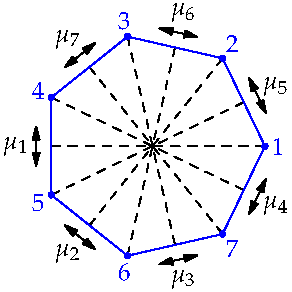
\includegraphics{perm-heptagon}\\
				$\rho_1=(1\,2\,3\,4\,5\,6\,7)$,\ \ $\rho_j=\rho_1^j$
			\end{tabular}
		\end{minipage}
		
		
		\item State the elements of the rotation group $R_5$ in cycle notation when viewed as a subgroup of $S_5$.
	  
	  
	  \item Prove parts 2, 3, and 4 of Lemma \ref{lemm:sabasic}.
	  
	  
	  \item How many distinct subgroups of $S_4$ are isomorphic to $S_3$. Describe them.
	  
		
	  \item\label{exs:symmwd} Suppose sets $A$ and $B$ have the same cardinality: that is, $\exists \mu:A\to B$ bijective.
	  \begin{enumerate}
	    \item If $\sigma\in S_A$ is a permutation, show that $\mu\sigma\mu^{-1}\in S_B$.
	    \item Hence prove that $S_A$ and $S_B$ are isomorphic.
	  \end{enumerate}
	  
	  
	  \item Cayley's Theorem says that $G$ is isomorphic to a subgroup of $S_G$.  What can you say about a (finite) group $G$ if $G\cong S_G$?
	
	  
	  \item In Cayley's Theorem we defined $\phi(g)=L_g:G\to G$ via \emph{left-multiplication.}
	  \begin{enumerate}
	    \item Does the argument still work if $\phi(g)=R_g:G\to G$ is \emph{right-multiplication} $R_g(x)=xg$?
	    
	    \item (Harder)\lstsp Suppose we take $\phi(g)=C_g:G\to G$ to be the function $C_g(z)=gx g^{-1}$. Does the proof of Cayley's Theorem work this time? Why/why not?
	  \end{enumerate}
		
		
		\item Show that the group $S_3$ is \emph{indecomposable}: there are no groups $G,H$ of order less than $\nm{S_3}=6$ for which $S_3\cong G\times H$.\par
		(\emph{Hint: Assuming $S_3$ is decomposable, there is only one possible decomposition. Why does this decomposition make no sense?})
	  
	  
	  \item\label{exs:centerSn} Let $n\ge 3$. Prove that if $\sigma\in S_n$ commutes with every other element of $S_n$ (i.e. $\sigma\rho=\rho\sigma,\ \forall \rho\in S_n$) then $\sigma$ is the identity.\par
	  (\emph{Hint: suppose $\sigma(a)=b\neq a$ and consider the cases $\sigma(b)=a$ and $\sigma(b)\neq a$ separately})
	
	\end{enumerate}
\end{exercises}


\clearpage


\subsection{Orbits}\label{sec:orbits}

Group theory is often applied by allowing the elements of a group to transform a set.\footnote{The formal definition of such \emph{group actions} is postponed until Chapter \ref{chap:action}.} We've already seen several examples: for instance, how rotations transform a geometric figure. The simplest general example is built into the definition of the symmetric group and appears naturally in cycle notation.

\begin{defn}{}{}
	The \emph{orbit} of $\sigma\in S_n$ containing $x\in\{1,2,\ldots,n\}$ is the \emph{set}
	\[
		\orb_x(\sigma)=\{\sigma^k(x):k\in\Z\}\subseteq\{1,2,\ldots,n\}
	\]
\end{defn}

\textcolor{red}{Warning!} Each orbit is a subset of $\{1,2,\ldots,n\}$, \emph{not} of the group $S_n$.\smallbreak
Observe also that $\orb_{\sigma^k(x)}(\sigma)=\orb_x(\sigma)$ for any $k\in\Z$.


\begin{examples}{}{}
	If $\sigma\in S_n$ is written as a product of \emph{disjoint cycles,} then the cycles are the orbits.
	\begin{enumerate}
	  \item The orbits of $(1\,3\,4)\in S_4$ are the disjoint sets $\{1,3,4\},\{2\}$. Note the singleton orbit $\{2\}$!
	  \item The orbits of $(1\,2)(4\,5)\in S_5$ are $\{1,2\},\{3\},\{4,5\}$.
	  \item Non-disjoint cycles are not orbits. For instance, $\sigma=(1\,3)(2\,3\,4)\in S_4$ maps
		\[
			1\mapsto 3\mapsto 4\mapsto 2\mapsto 1
		\]
		so there is only one orbit: $\orb_x(\sigma)=\{1,2,3,4\}$ for any $x$. This comports with the result obtained by multiplying cycles via the usual algorithm: $\sigma=(1\,2\,3\,4)$.
	\end{enumerate}
\end{examples}

Given that disjoint cycle notation is so useful for reading orbits, it is natural to ask if \emph{any} permutation can be written in such a manner. The answer is yes, as we demonstrate in the next two results.


\begin{lemm}{}{orbit}
	The orbits of $\sigma\in S_n$ partition $X=\{1,2,\ldots,n\}$.
\end{lemm}

\begin{proof}
	Define a relation $\sim$ on $X=\{1,2,\ldots,n\}$ by $x\sim y\iff y\in\orb_x(\sigma)$. We claim that this is an equivalence relation.\footnotemark
	\begin{quote}
	\begin{description}
		\item[\normalfont\emph{Reflexivity}] $x\sim x$ since $x=\sigma^0(x)$. \checkmark
		\item[\normalfont\emph{Symmetry}] $x\sim y\implies y=\sigma^k(x)$ for some $k\in\Z$. But then $x=\sigma^{-k}(y) \implies y\sim x$. \checkmark
		\item[\normalfont\emph{Transitivity}] Suppose that $x\sim y$ and $y\sim z$. Then $y=\sigma^k(x)$ and $z=\sigma^l(y)$ for some $k,l\in\Z$. But then $z=\sigma^{k+l}(x)$ and so $x\sim z$. \checkmark
	\end{description}
	\end{quote}
	The equivalence classes of $\sim$ are clearly the orbits of $\sigma$, which therefore partition $X$.
\end{proof}

\footnotetext{%
	The relationship between equivalence relations and partitions underpins several upcoming ideas, and \emph{should} be familiar from a previous course. Here is a very quick review:\smallbreak
	Given $x\in X$ and a relation $\sim$ on $X$, define the set $[x]:=\{y\in X:y\sim x\}$.\smallbreak
  Theorem: The sets $[x]$ \emph{partition} $X$ (every $y\in X$ lies in precisely one such subset $[x]$) if and only if $\sim$ is an \emph{equivalence relation} (reflexive, symmetric, transitive). In such a case we call $[x]$ an \emph{equivalence class.}\smallbreak
  In our situation, $[x]=\orb_x(\sigma)$; the Lemma simply proves that the orbits of $\sigma$ are equivalence classes.
}

\goodbreak

\begin{thm}{}{cycleterminates}
	Every permutation can be written as a product of disjoint cycles.
\end{thm}

\begin{proof}
	We formalize the algorithm from page \pageref{pg:cyclenot}. Suppose $\sigma\in S_n$ is given.
	\begin{enumerate}\itemsep0pt
	  \item List the elements of $\orb_{1}(\sigma)$ in the order they appear within the orbit:
		\[
			\orb_{1}(\sigma)=\{1,\sigma(1),\sigma^2(1),\ldots\}
		\]
		If this all of $X=\{1,\ldots,n\}$, we are finished: $\sigma=(1\ \sigma(1)\ \sigma^2(1)\ \ldots\ \sigma^{n-1}(1)\bigr)$ is an $n$-cycle.
		
		\item Otherwise, let $x_2=\min\{x\in X:x\not\in\orb_1(\sigma)\}$ and construct its orbit:
		\[
			\orb_{x_2}(\sigma)=\{x_2,\sigma(x_2),\sigma^2(x_2),\ldots\}
		\]
		By Lemma \ref{lemm:orbit}, $\orb_{x_2}(\sigma)$ is disjoint with $\orb_1(\sigma)$. If $\orb_{1}(\sigma)\cup\orb_{x_2}(\sigma)=X$ then we are done, and $\sigma$ is the product of two disjoint cycles:
		\[
			\sigma=\bigl(1\ \sigma(1)\ \sigma^2(1)\ \cdots\bigr)\bigl(x_2\ \sigma(x_2)\ \sigma^2(x_2)\ \cdots\bigr)
		\]
		
		\item Otherwise, repeat. At stage $k$, let $x_k=\min\{x\in X:x\not\in\orb_1(\sigma)\cup\cdots\cup\orb_{k-1}(\sigma)\}$. By the Lemma, $\orb_{x_k}(\sigma)$ is disjoint with $\orb_1(\sigma)\cup\cdots\cup\orb_{k-1}(\sigma)$. The process continues until $\orb_1(\sigma)\cup\cdots\cup\orb_{k}(\sigma)=X$, which must happen eventually since $X$ is a finite set. The result is a product of disjoint cycles:
		\[
			\def\phan{\makebox[0pt][c]{\phantom{$\sigma^2(x_1)$}}}
			\sigma=\bigl(\underbrace{1\ \sigma(1)\ \phan\sigma^2(1)\ \cdots}_{\orb_1(\sigma)}\bigr)\bigl(\underbrace{x_2\ \sigma(x_2)\ \sigma^2(x_2)\ \cdots}_{\orb_{x_2}(\sigma)}\bigr)\bigl(\underbrace{\cdots\phan\cdots}_{\orb_{x_3}(\sigma)}\bigr)\cdots\bigl(\underbrace{\cdots\phan\cdots}_{\orb_{x_k}(\sigma)}\bigr) \tag*{\qedhere}
		\]
	\end{enumerate}
\end{proof}

The Theorem explains why our cycle algorithm always produces a product of disjoint cycles! By convention, $1<x_2<\cdots<x_k$, though there is no need to do this: disjoint cycles can be listed in any order and may start with any element, e.g.,
\[
	(1\,3)(2\,5\,4)=(5\,4\,2)(3\,1)
\]
Also, by convention, we delete any orbits of size 1 (1-cycles). %If you are still feeling uncomfortable multiplying cycles, practice until it becomes second-nature!

\vfil

\boldsubsubsection{Orders of Elements in $S_n$}

Recall (Corollary \ref{cor:orderdefn}) that the order of an element $\sigma\in S_n$ is the smallest positive integer $k$ for which $\sigma^k=e$.

\begin{example}[lower separated=false, sidebyside, sidebyside align=top seam, sidebyside gap=0pt, righthand width=0.22\linewidth]{}{}
	If $\sigma=(1\,2\,3\,4\,5\,6)\in S_6$, then
	\begin{align*}
		&\sigma^2=(1\,3\,5)(2\,4\,6) &&\sigma^3=(1\,4)(2\,5)(3\,6) &&\sigma^4=(1\,5\,3)(2\,6\,4)\\
		&\sigma^5=(1\,6\,5\,4\,3\,2) &&\sigma^6=e&&
	\end{align*}
	whence the order of $\sigma$ is 6. This is intuitive if we identify $\sigma$ with a counter-clockwise rotation of a regular hexagon: indeed $\ip{\sigma}=\{e,\sigma,\ldots,\sigma^5\} \cong R_6$.
	\tcblower
	\flushright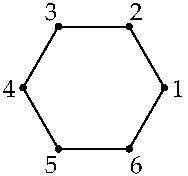
\includegraphics{perm-hexagon}
\end{example}

By similarly considering a regular $k$-gon, it should be clear that every $k$-cycle has order $k$.

\goodbreak

Things are trickier when you don't have a single cycle. However, we are again saved by the discussion of disjoint cycles, since \emph{disjoint cycles commute.}

\begin{examples}{}{}
	\exstart Since $(1\,2\,3)$ and $(4\,5)$ are disjoint cycles, we know that $(1\,2\,3)(4\,5)=(4\,5)(1\,2\,3)$. We therefore easily compute
		\begin{align*}
			\bigl((1\,2\,3)(4\,5)\bigr)^3&=(1\,2\,3)(4\,5)(1\,2\,3)(4\,5)(1\,2\,3)(4\,5)\\
			&=(1\,2\,3)^3(4\,5)^3 =e(4\,5)=(4\,5)
		\end{align*}
	\begin{enumerate}\setcounter{enumi}{1}
		\item Given $\sigma=(2\,5\,3)(1\,5\,4\,3)\in S_5$, we find $\sigma^{8}$. It is tempting to write
		\[
			\sigma^{8}\overset{\text{?}}{=}(2\,5\,3)^{8}(1\,5\,4\,3)^{8} =\bigl((2\,5\,3)^3\bigr)^2(2\,5\,3)^2\bigl((1\,5\,4\,3)^4\bigr)^2 =e^3(2\,3\,5)e^2  =(2\,3\,5)
		\]
		but this would be incorrect: the \emph{cycles don't commute} $(2\,5\,3)(1\,5\,4\,3)\neq (1\,5\,4\,3)(2\,5\,3)$ so we cannot distribute the exponent (8). If instead we first find $\sigma$ as a product of disjoint cycles, then the exponent does distribute and the computation is easy
		\[
			\sigma=(1\,3)(2\,5\,4)\implies \sigma^8=(1\,3)^8(2\,5\,4)^8=(2\,5\,4)^2 =(2\,4\,5)
		\]
		This approach also tells us the order of $\sigma$. Observe that
		\[
			e=\sigma^k=(1\,3)^k(2\,5\,4)^k\iff k\text{ is divisible by both 2 and 3}
		\]
		The order if $\sigma$ is therefore 6.
	\end{enumerate}
\end{examples}

\begin{cor}{}{}
	The order of a permutation $\sigma$ is the least common multiple of the lengths of its disjoint cycles.
\end{cor}

\begin{proof}
	Write $\sigma=\sigma_1\cdots\sigma_m$ as a product of disjoint cycles, where the cycle $\sigma_j$ has length $\alpha_j$. Since disjoint cycles commute,
	\[
		\sigma^k=\sigma_1^k\cdots\sigma_m^k
	\]
	Since each factor $\sigma_j^k$ permutes disjoint sets, it follows that
	\[
		\sigma^k=e\iff\forall j,\ \sigma_j^k=e \iff \forall j, \ \alpha_j\mid k \tag{the order of an $\alpha_j$-cycle is $\alpha_j$}
	\] 
	The order of $\sigma$ is the smallest $k$ satisfying this condition, namely $\lcm(\alpha_1,\ldots,\alpha_m)$.
\end{proof}

\begin{example}{}{}
	Since $\sigma=(1\,4\,5)(3\,6\,2\,7)(8\,9)\in S_9$ is written as a product of disjoint cycles, its order is $\lcm(3,4,2)=12$.\smallbreak
	To compute $\sigma^{3465}$, first observe that $3465=12\cdot 288+9$ (division algorithm). From this,
	\[
		\sigma^{3465}=(\sigma^{12})^{288}\sigma^9=\sigma^9=(1\,4\,5)^9(3\,6\,2\,7)^9(8\,9)^9=(3\,6\,2\,7)(8\,9)
	\]
	since $(1\,4\,5)$, $(3\,6\,2\,7)$ and $(8\,9)$ have orders 3, 4 and 2 respectively.
\end{example}

\goodbreak

\begin{exercises}
	Key concepts:\quad
		\emph{Orbit \quad Partition \quad Disjoint cycles \quad Order of element via lcm}
	
	\begin{enumerate}
	  \item Find the orbits of the following permutations, and their orders:
	  \begin{enumerate}
	    \item $\rho=(1\,4\,5)(2\,3\,4\,5)\in S_5$.
	    \item $\sigma=(1\,5\,4)(2\,5\,4)(1\,2\,3\,4)\in S_5$.
	    \item $\tau=(1\,5\,7\,4)(3\,2\,4)(3\,2\,5\,6)\in S_7$.
	  \end{enumerate}
	
	
	  \item If $\sigma\in S_A$ is any permutation, we may define its orbits similarly: $\orb_a(\sigma)=\{\sigma^j(a):j\in\Z\}$. What are the orbits of the permutation $\sigma:\Z\to\Z:n\mapsto n+3$?
	  
		
		\item Given $\sigma=(1\,3)(2\,4\,5)\in S_5$, find the elements of the cyclic group $\ip\sigma\le S_5$ generated by $\sigma$.
		
		
		\item What is the largest possible order of an element of the group $S_3\times\Z_4\times V$? Exhibit one.
	
	
		\item What is the maximum order of an element in each of the groups $S_4,S_5,S_6,S_7,S_8$? Exhibit a maximum order element in each case.
		
	
		\item For which integers $n$ does there exist a subgroup $C_n\le S_8$ where $C_n$ is cyclic of order $n$? Explain your answer.
		
	
	 	\item Let $\sigma\in S_n$. For each $k>0$, prove that each orbit of $\sigma^k$ is a subset of an orbit of $\sigma$.
	 	
	
		\item Consider the permutations $\sigma=(1\,3\,5)(2\,7\,4\,9\,6)$ and $\tau=(1\,5\,3\,2)(6\,9)$ in $S_9$.
	  \begin{enumerate}
	      \item Compute $\sigma\tau$ and $\tau\sigma$ in cycle notation.
	      \item Find the orders of $\sigma$, $\tau$, $\sigma\tau$ and $\tau\sigma$.
	      \item Compute $(\sigma\tau)^{432}\sigma^{43}$ as a product of disjoint cycles.
				\item Construct the subgroup diagram of $\ip{\sigma}$ and give a generator for each subgroup.
	  \end{enumerate}
	  
	\end{enumerate}
\end{exercises}


\clearpage


\subsection{Transpositions \& the Alternating Group}\label{sec:transpositions}

In the previous sections we viewed a permutation in terms of its orbits. An alternative approach involves the construction of permutation from the very simplest bijections.

\begin{defn}{}{}
	A 2-cycle $(a_1\,a_2)$ is also known as a \emph{transposition,} since it swaps two elements of $\{1,2,\ldots,n\}$ and leaves the rest untouched.
\end{defn}


\begin{thm}{}{}
	Every $\sigma\in S_n$ ($n\ge 2$) may be written as a product of transpositions.
\end{thm}

\begin{proof}
	There are many, many ways to do this. One approach is first to write $\sigma$ as a product of disjoint cycles, before decomposing each cycle as follows:
	\[
		(a_1\,\cdots\, a_k)=(a_1\,a_k)(a_1\,a_{k-1})\cdots (a_1\,a_2)
	\]
	Just read carefully and you should be convinced this works!
\end{proof}

\begin{example}{}{}
	The method in the proof results in the decomposition
	\[
		(1\,7\,6\,4\,5)=(1\,5)(1\,4)(1\,6)(1\,7)
	\]
	Other decompositions are possible, for instance $(1\,7)(3\,6)(5\,7)(4\,7)(3\,6)(6\,7)$.
\end{example}

While representations as a product of transpositions are non-unique, a simple commonality may easily be observed via a \emph{matrix notation.} Consider, for instance,
\[
	\begin{pmatrix}
		1&0&0&0\\ 0&0&0&1\\ 0&0&1&0\\ 0&1&0&0
	\end{pmatrix}
	\fourvec 1234
	=\fourvec 1432\quad\text{and}\quad
	\begin{pmatrix}
		0&0&1&0\\ 0&0&0&1\\  0&1&0&0\\ 1&0&0&0
	\end{pmatrix}
	\fourvec 1234
	=\fourvec 3421\tag{$\ast$}
\] 
Each of these $4\times 4$ matrices \emph{permutes} the values 1, 2, 3, 4 when placed in a column vector. The matrices plainly correspond to the transposition $(2\,4)$ and the 4-cycle $(1\,3\,2\,4)$ in $S_4$.

\begin{defn}{}{}
	An $n\times n$ \emph{permutation matrix} is a matrix obtained from the identity matrix by permuting its \emph{rows.} Equivalently, it is zero except for a single 1 in each row and column.
\end{defn}

\begin{lemm}{}{}
	The set of $n\times n$ permutation matrices forms a multiplicative group isomorphic to $S_n$.
\end{lemm}

We omit a formal proof, though it relies on essentially one fact from elementary linear algebra: that \emph{row operations} preserve the solution set of a system of linear equations. For instance $(\ast)$ describes two linear systems $A\vx=\vb$ and $C\vx=\vd$ with identical solutions $\vx$, differing only by row operations.
\smallbreak

What does this have to do with transpositions? Since a transposition swaps two elements, it corresponds to multiplication by a \emph{row-swapping elementary matrix}; any such matrix has determinant $-1$. Suppose that a permutation is written as a product of transpositions:
\[
	\sigma=\sigma_1\cdots\sigma_m
\]
and view this as a product of matrices, taking determinant of both sides shows that
\[
	\det\sigma=(-1)^m
\]
The value of the determinant plainly depends only on whether $m$ is \emph{even} or \emph{odd}\ldots

\begin{defn}{}{}
	A permutation $\sigma\in S_n$ is \emph{even}/\emph{odd} if it can be written as the product of an even/odd number of transpositions.
\end{defn}

By our matrix/determinant discussion, the parity of a permutation is well-defined: every permutation is either even or odd; it cannot be both!\smallbreak

Plainly the composition of even permutations remains even, as does the inverse of such. We may therefore define a new subgroup of $S_n$.

\begin{defn}{}{}
	The \emph{alternating group} $A_n$ ($n\ge 2$) is the group of even permutations in $S_n$.
\end{defn}

\begin{thm}{}{alt}
	$A_n$ contains exactly half the elements of $S_n$: otherwise said, $\nm{A_n}=\frac{n!}{2}$.
\end{thm}

\begin{proof}
	Since $n\ge 2$, we have $(1\,2)\in S_n$. Define $\phi:S_n\to S_n$ by $\phi(\sigma)=(1\,2)\sigma$. Since
	\[
		(1\,2)(1\,2)\sigma=\sigma
	\]
	we see that $\phi$ is invertible ($\phi$ is its own inverse!). Moreover, $\phi$ maps even permutations to odd and vice versa. It follows that there are exactly the same number of odd and even permutations.
\end{proof}

\begin{examples}{}{tetra}
	We describe the smallest three alternating groups $A_4$.
	\begin{enumerate}
	  \item $A_2=\{e\}\cong \Z_1$ is trivial.
	  \item $A_3=\{e,\,(1\,3)(1\,2)\,,(1\,2)(1\,3)\}=\{e,\,(1\,2\,3),\,(1\,3\,2)\}\cong\Z_3$ is a cyclic group.
	  \item\label{ex:tetra2} When $n=4$ we obtain the first `new' group in the alternating family; a group of order 12.
	  \begin{align*}
	  	A_4=\{e,\,(1\,2\,3),\,(1\,3\,2),\,&(1\,2\,4),\,(1\,4\,2),\,(1\,3\,4),\,(1\,4\,3),\,(2\,3\,4),\,(2\,4\,3),\\
	  	&(1\,2)(3\,4),\,(1\,3)(2\,4),\,(1\,4)(2\,3)\}
	  \end{align*}
	  \begin{minipage}[t]{0.69\linewidth}\vspace{0pt}
	    $A_4$ is non-abelian: for example,
	  	\[
	  		(1\,2\,3)(1\,2\,4)=(1\,3)(2\,4)\neq (1\,4)(2\,3)=(1\,2\,4)(1\,2\,3)
	  	\]
	  	While we've already countered one non-abelian group of order 12, the dihedral group $D_6$, we quickly see that $A_4\ncong D_6$: all elements of $A_4$ have orders 1, 2 or 3, while $D_6$ contains a rotation (by $\ang{60}$) of order 6.\smallbreak
	  By labelling faces (or vertices), $A_4$ may be visualized the 3D-rotation group of a regular tetrahedron: can you see how each element acts?
	  \end{minipage}
	  \hfill
	  \begin{minipage}[t]{0.3\linewidth}\vspace{0pt}
	  	\flushright\href{https://www.math.uci.edu/~ndonalds/math120a/perm-a4.html}{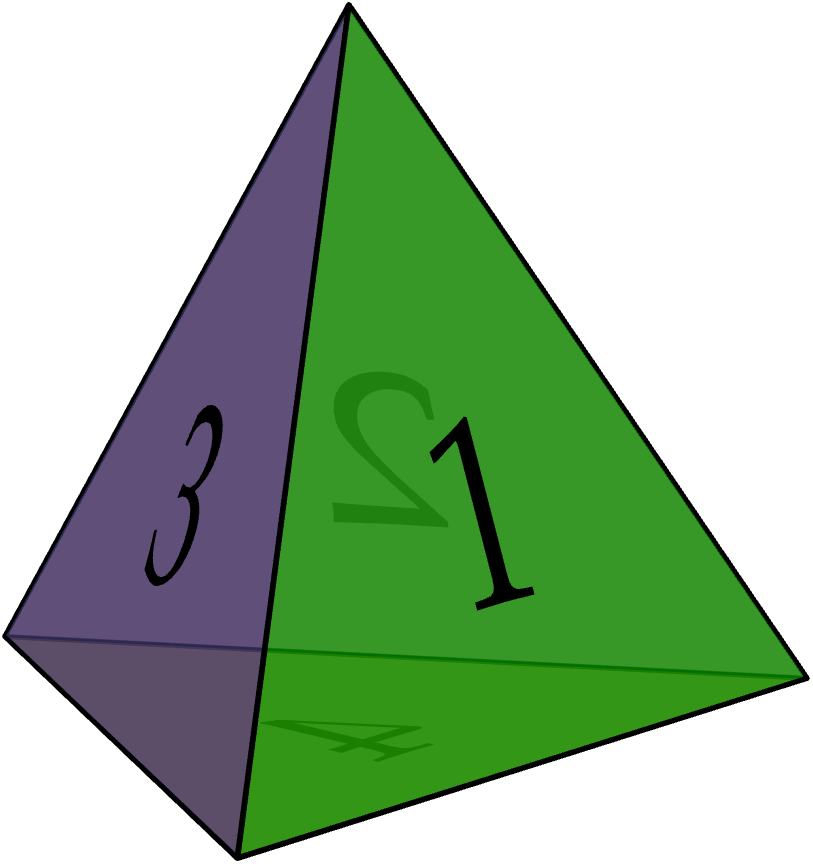
\includegraphics[scale=0.14]{perm-a4.png}}
	  \end{minipage}
	
	\end{enumerate}
\end{examples}


\begin{exercises}
	Key concepts:\quad
	%\begin{quote}
		\emph{Transposition (representation of elements)\quad Odd/even permutations\quad $A_n$}
	%\end{quote}
	
	\begin{enumerate}
	  \item Write $(1\,3\,4\,6)(2\,4\,6)$ as a product of transpositions in two different ways.
	  
	  
	  \item State $\sigma=(1\,3)$ and $\tau=(1\,3\,2)$ as $3\times 3$ permutation matrices $S$ and $T$. Compute the matrix product $ST$ and verify that it is the permutation matrix corresponding to $\sigma\tau\in S_3$.
	  
	  
	  \item Give examples of two non-isomorphic non-abelian groups of order 360.
	  
	  
	  \item Explain why every finite group is isomorphic to a group of matrices under multiplication.
	  
	  
	  \item $S_4$ has \emph{four} distinct subgroups isomorphic to the Klein four-group $V$; state them. Only one of these is a subgroup of $A_4$; which?
	  
	  
	  \item We just saw that the rotation group of a regular tetrahedron is isomorphic to $A_4$.
	  \begin{enumerate}
	    \item What is the order of the rotation group of a cube?\par
	    (\emph{Hint: each face may be rotated to any of six faces, and then rotated in place\ldots})
	    
	    \item Repeat the calculation for the remaining three platonic solids (octahedron, dodecahedron, icosahedron).
	    
	    \item By placing a vertex at the center of each face of a cube, argue that the rotation group of an octahedron is also isomorphic to $S_4$.\par
	    What happens when you do this for a dodecahedron? A tetrahedron?
	    
	    \item Label the four diagonals of a cube 1, 2, 3, 4. Describe geometrically the effect of the permutation $(2\,3\,4)$ on the cube. What about $(2\,3)$? Hence conclude that the rotation group of a cube is isomorphic to $S_4$.\par
	    (\emph{The dodecahedral and icosahedral rotation groups are both isomorphic to the alternating group $A_5$, though this is harder to visualize than the cube situation---try researching a proof\ldots})
	  \end{enumerate}
	  
	  	
	 	\item\label{exs:a4subgroups} (Hard) Find the entire subgroup diagram of $A_4$.
	 	
	  
	  \item (Hard) Prove that $D_n$ is a subgroup of $A_n\iff n\equiv 1\pmod 4$\par
		(\emph{Do this in one shot if you like; otherwise use the following steps to guide your thinking})
		\begin{enumerate}
	   	\item Label the corners of a regular $n$-gon 1 through $n$ counter-clockwise so that every element of $D_n$ may be written as a permutation of $\{1,2,\ldots,n\}$. Write in a sentence what you are required to prove: what condition characterizes being in the group $A_n$?
	   	
	   	\item Consider the rotation $\rho_1=(1\,2\,3\,\cdots \,n)$ of the $n$-gon one step counter-clockwise. Is $\rho_1$ odd or even, and how does this depend on $n$?
	   	
	   	\item Show that every rotation $\rho_i\in D_n$ is generated by $\rho_1$. When is the set of rotations in $D_n$ a subgroup of $A_n$?
	   	
	   	\item A reflection $\mu\in D_n$ permutes corners of the $n$-gon by swapping pairs. How many pairs of corners does $\mu$ swap when $n\equiv 1\pmod 4$? Is $\mu$ an odd or even permutation? You may use a picture, provided it is sufficiently general.
	   	
	   	\item Summarize parts (a--d) to argue the $\Leftarrow$ direction of the theorem.
	   	
	   	\item Prove the $\Rightarrow$ direction of the theorem by exhibiting an element of $D_n$ which is not in $A_n$ whenever $n\not\equiv 1\pmod 4$.
	\end{enumerate}
	
	
	\end{enumerate}
\end{exercises}
